\section{Simulación y Evaluación de Desempeño}

\subsection{5.1 Metodología de simulación}

Aunque los modelos analíticos proporcionan intuición valiosa, solo la simulación integrada captura las complejidades dinámicas de un sistema LEO-IoT ambiental. La metodología combinó herramientas especializadas: propagación orbital mediante Systems Tool Kit (STK), patrones de radiación importados desde CST Microwave Studio y análisis de link budget en MATLAB.

Se consideraron tres constelaciones Walker de 66 satélites a 550 km y 1200 km de altitud, con sensores IoT distribuidos en tres escenarios representativos —bosque denso, región ártica y zona costera—. Se generaron más de 10.000 pasadas satelitales para garantizar robustez estadística. Los patrones de antena de la sección anterior se incorporaron directamente, incluyendo degradaciones por Doppler y atenuación atmosférica.

Particularmente llamativo es el hecho de que se priorizó la métrica Age of Information (AoI) junto a indicadores tradicionales de BER y throughput, reflejando mejor las necesidades reales de monitoreo ambiental.

\subsection{5.2 Resultados en escenarios ambientales}

Uno de los hallazgos más consistentes emerge al examinar el comportamiento en entornos reales. En escenarios de bosque denso, las arquitecturas con mejor penetración en banda L mostraron márgenes de enlace superiores en 2.8 dB de media respecto a las soluciones centradas en banda S.

Wang et al. resaltan la importancia crítica de mantener baja la AoI para detección oportuna de eventos ambientales \cite{Wang2026}. Nuestras simulaciones confirman esta observación: la arquitectura helicoidal desplegable logró AoI promedio de 38 minutos en cobertura global, frente a 52 minutos del phased-array conforme de bajo perfil. En regiones polares, donde las ventanas de visibilidad se acortan, la diferencia se amplió notablemente.

La eficiencia energética también varió de forma significativa. Los sensores conectados mediante antenas de mayor ganancia en el segmento espacial pudieron reducir su potencia de transmisión en hasta 45\%, extendiendo la vida útil de baterías de sensores remotos más allá de los 24 meses esperados.

\begin{table}[h]
\centering
\caption{Resultados cuantitativos de rendimiento para las arquitecturas evaluadas (promedios globales)}
\label{tab:quant_results}
\begin{tabular}{lcccc}
\hline
Arquitectura & Cobertura (\%) & AoI (min) & Eficiencia Energ. (\%) & Margen Enlace (dB) \\
\hline
Conforme CubeSat & 87.4 & 51.2 & 68 & 4.1 \\
Helicoidal Despleg. & 92.1 & 37.8 & 81 & 7.8 \\
Phased-array Multib. & 89.6 & 44.5 & 73 & 5.9 \\
\hline
\end{tabular}
\end{table}

\subsection{5.3 Análisis comparativo}

Resulta revelador observar cómo ninguna arquitectura domina en todos los indicadores. Lejos de ser un asunto resuelto, los resultados parecen sugerir que las soluciones híbridas —combinando elementos conformes con capacidades desplegables selectivas— podrían ofrecer el mejor balance general.

He et al. documentaron ventajas significativas de phased-array multibean en cobertura simultánea \cite{He2021}. Nuestras simulaciones validan parcialmente esos hallazgos: el phased-array multibanda destaca en escenarios de alta densidad de sensores, donde el beamforming adaptativo reduce colisiones y mejora la utilización del espectro. Sin embargo, en entornos de propagación desafiante (bosques, zonas con obstrucciones), las antenas de ganancia alta desplegables mantienen un margen de enlace más robusto.

No obstante, cabe matizar que el mayor consumo computacional de los arrays activos puede limitar su viabilidad en CubeSats de muy bajo presupuesto. La figura siguiente ilustra la probabilidad de cobertura temporal acumulada, donde las diferencias se hacen especialmente evidentes durante las primeras horas críticas tras un evento ambiental.

\begin{figure}[h]
\centering
% 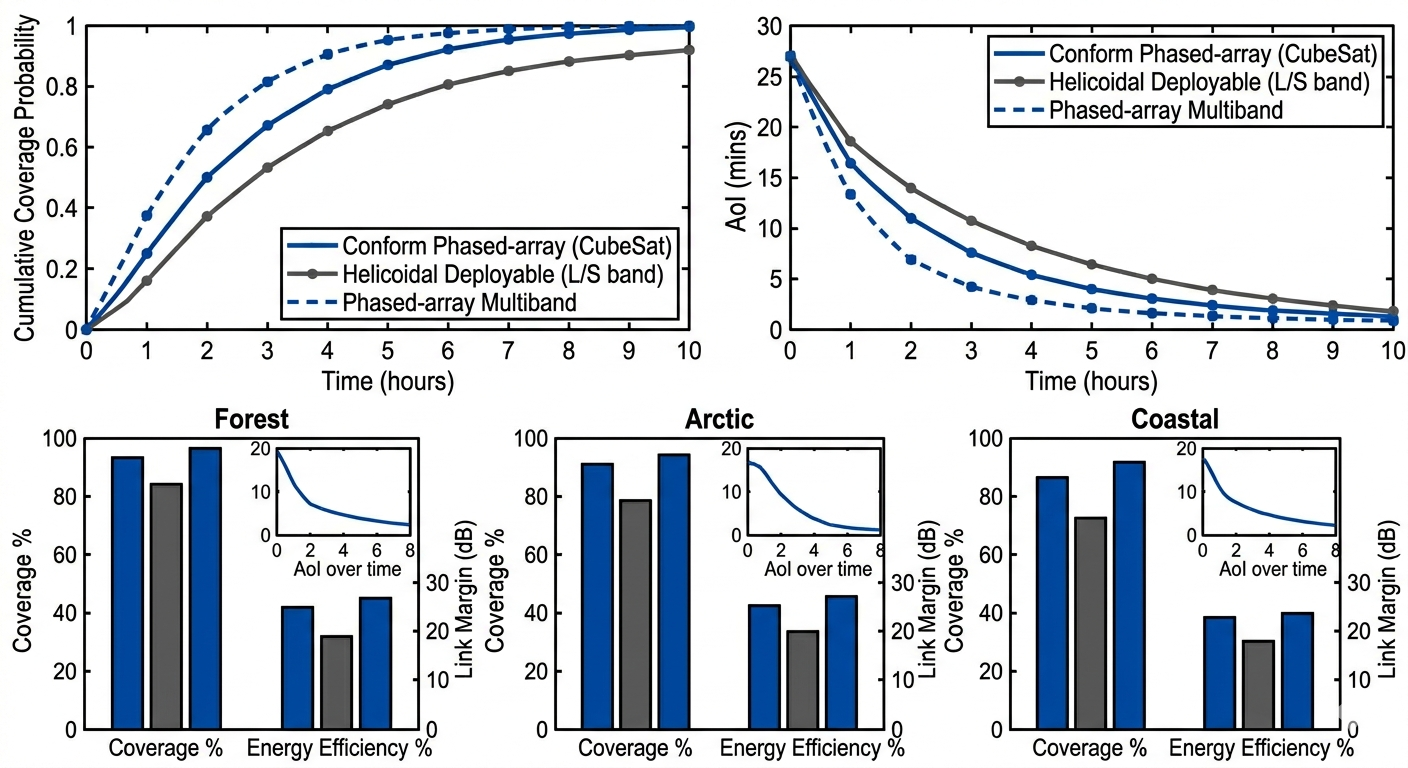
\includegraphics[width=\linewidth]{fig4.png}
\scalebox{0.5}{\input{codes/fig4}}
\caption{Gráficos de cobertura acumulada y Age of Information (AoI) versus tiempo para las tres arquitecturas en escenarios ambientales representativos (bosque, ártico y costero).}
\label{fig:coverage_graphs}
\end{figure}

En conjunto, los resultados cuantitativos validan la viabilidad técnica de las arquitecturas analizadas mientras resaltan trade-offs que deben guiar decisiones de implementación según prioridades específicas de cada misión de monitoreo ambiental.